\documentclass[letterpaper,12pt]{article}
\usepackage{array}
\usepackage{threeparttable}
\usepackage{fancyhdr,lastpage}
\pagestyle{fancy}
\lhead{}
\chead{}
\rhead{}
\lfoot{}
\cfoot{}
\rfoot{\footnotesize\textsl{Page \thepage\ of \pageref{LastPage}}}
\renewcommand\headrulewidth{0pt}
\renewcommand\footrulewidth{0pt}
\usepackage[format=hang,font=normalsize,labelfont=bf]{caption}
\usepackage{listings}
\lstset{frame=single,
  language=Python,
  showstringspaces=false,
  columns=flexible,
  basicstyle={\small\ttfamily},
  numbers=none,
  breaklines=true,
  breakatwhitespace=true
  tabsize=3
}

\usepackage{geometry}
\geometry{letterpaper,tmargin=1in,bmargin=1in,lmargin=1in,rmargin=1in}
%\renewcommand\headrulewidth{2pt}
%\renewcommand\footrulewidth{2pt}
\usepackage{amsmath}
\usepackage{amssymb}
\usepackage{amsthm}
\usepackage{mathtools}
\usepackage{pdflscape}
\usepackage{harvard}
\usepackage{setspace}
\usepackage{float,color}
%\usepackage{enumitem}
\usepackage[pdftex]{graphicx}
\usepackage{hyperref}
\hypersetup{colorlinks,linkcolor=red,urlcolor=blue}
\theoremstyle{definition}
\newtheorem{theorem}{Theorem}
\newtheorem{acknowledgement}[theorem]{Acknowledgement}
\newtheorem{algorithm}[theorem]{Algorithm}
\newtheorem{axiom}[theorem]{Axiom}
\newtheorem{case}[theorem]{Case}
\newtheorem{claim}[theorem]{Claim}
\newtheorem{conclusion}[theorem]{Conclusion}
\newtheorem{condition}[theorem]{Condition}
\newtheorem{conjecture}[theorem]{Conjecture}
\newtheorem{corollary}[theorem]{Corollary}
\newtheorem{criterion}[theorem]{Criterion}
\newtheorem{definition}[theorem]{Definition}
\newtheorem{derivation}{Derivation} % Number derivations on their own
\newtheorem{example}[theorem]{Example}
\newtheorem{exercise}[theorem]{Exercise}
\newtheorem{lemma}[theorem]{Lemma}
\newtheorem{notation}[theorem]{Notation}
\newtheorem{problem}[theorem]{Problem}
\newtheorem{proposition}{Proposition} % Number propositions on their own
\newtheorem{remark}[theorem]{Remark}
\newtheorem{solution}[theorem]{Solution}
\newtheorem{summary}[theorem]{Summary}
\numberwithin{equation}{section}
\bibliographystyle{aer}
\newcommand\ve{\varepsilon}
\newcommand\boldline{\arrayrulewidth{1pt}\hline}
\newcommand{\q}[1]{``#1''}

\def\changemargin#1#2{\list{}{\rightmargin#2\leftmargin#1}\item[]}
\let\endchangemargin=\endlist 

\usepackage{graphicx}
\graphicspath{ {images/} }

\usepackage{enumerate}
%\usepackage[shortlabels]{enumerate}
\setlength{\parindent}{24pt}
%\renewcommand{\baselinestretch}{2.0}
\usepackage{lipsum} % just for the example
\makeatletter
\newcommand{\verbatimfont}[1]{\renewcommand{\verbatim@font}{\ttfamily#1}}
\makeatother
%\usepackage{enumitem}
\usepackage{float}

\verbatimfont{\small}%


\begin{document}

\begin{flushleft}
   \textbf{\Large{Problem Set \#4}} \\
   MACSS 30100 \\
   Xinzhu Sun, 12147991\\
\end{flushleft}

\noindent \textbf{\large Problem 1}\par

\begin{enumerate} [\bfseries (a)]
\item The following graph is the histogram of the income distribution of the MACSS graduates:\\
\begin{figure}[H]
\centering
\fbox{\resizebox{4.75in}{3in}{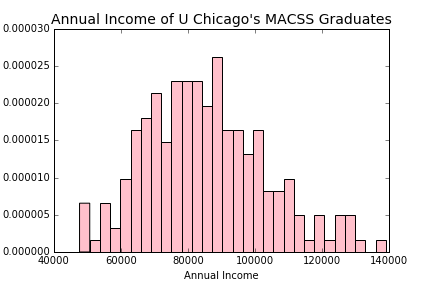
\includegraphics{Fig_1a}}}\
\end{figure}\par

\item The lognormal PDF value of the test matrix is:  [[ 0.0019079   0.00123533], [ 0.00217547  0.0019646 ]]. 
	
\item The following graph is the lognormal PDF of SMM against the income distribution histogram of he MACSS graduates:
\begin{figure}[H]
\centering
\fbox{\resizebox{5in}{3in}{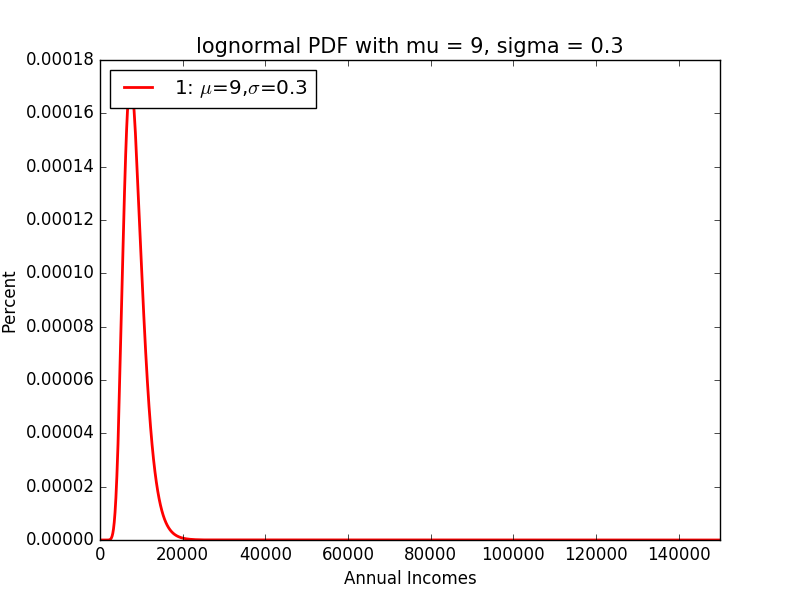
\includegraphics{Fig_1b}}}\
\end{figure}\par
The SMM lognormal parameters are: \(\mu = 11.3307147908, \, \sigma = 0.208868365237\). \\
The value of the SMM criterion function is \(8.82875694e-15\).\\
The data mean is 85276.8236063, the data standard deviation is 17992.542128.\\
The model mean is  85276.8301573 ,the model standard deviation is 17992.5416413.\\
The two data moments and model moments of SMM are almost the same.\par	

\item The following graph is the lognormal PDF of two-step SMM against the income distribution histogram and the lognormal PDF of one-step SMM of he MACSS graduates:
\begin{figure}[H]
\centering
\fbox{\resizebox{5in}{3in}{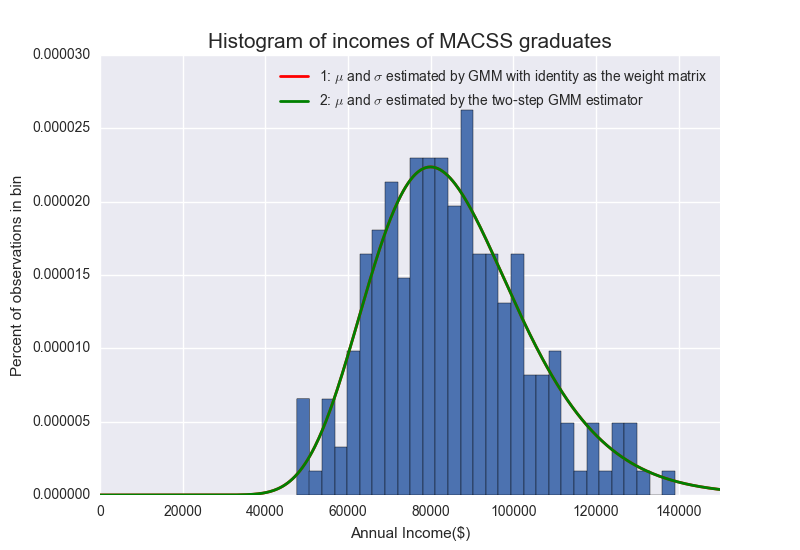
\includegraphics{Fig_1c}}}\
\end{figure}\par
The two-step SMM lognormal parameters are: \(\mu = 11.3307149281, \, \sigma = 0.208868373669\). \\
The value of the SMM criterion function is \(2.31293318e-07\).\\
The data mean is 85276.8236063, the data standard deviation is 17992.542128.\\
The model mean is  85276.8420177 ,the model standard deviation is 17992.5448859.\\
The two data moments and model moments of two-step SMM are almost the same.\par	

\end{enumerate}
\end{document}